%% ****** Start of file apstemplate.tex ****** %
%%
%%
%%   This file is part of the APS files in the REVTeX 4 distribution.
%%   Version 4.1r of REVTeX, August 2010
%%
%%
%%   Copyright (c) 2001, 2009, 2010 The American Physical Society.
%%
%%   See the REVTeX 4 README file for restrictions and more information.
%%
%
% This is a template for producing manuscripts for use with REVTEX 4.0
% Copy this file to another name and then work on that file.
% That way, you always have this original template file to use.
%
% Group addresses by affiliation; use superscriptaddress for long
% author lists, or if there are many overlapping affiliations.
% For Phys. Rev. appearance, change preprint to twocolumn.
% Choose pra, prb, prc, prd, pre, prl, prstab, prstper, or rmp for journal
%  Add 'draft' option to mark overfull boxes with black boxes
%  Add 'showpacs' option to make PACS codes appear
%  Add 'showkeys' option to make keywords appear
\documentclass[aps,prl,twocolumn,superscriptaddress,floatfix]{revtex4-1}
%\documentclass[aps,prl,preprint,superscriptaddress]{revtex4-1}
%\documentclass[aps,prl,reprint,groupedaddress]{revtex4-1}

% You should use BibTeX and apsrev.bst for references
% Choosing a journal automatically selects the correct APS
% BibTeX style file (bst file), so only uncomment the line
% below if necessary.

\usepackage{graphicx}
\usepackage[caption=false]{subfig}
\usepackage{braket}
\usepackage{mathtools}
\usepackage{color}
\graphicspath{{figures/}}
\DeclareMathOperator{\sinc}{sinc}

\begin{document}

% Use the \preprint command to place your local institutional report
% number in the upper righthand corner of the title page in preprint mode.
% Multiple \preprint commands are allowed.
% Use the 'preprintnumbers' class option to override journal defaults
% to display numbers if necessary
%\preprint{}

%Title of paper
\title{Amplitude sensing below the zero-point fluctuations with a two-dimensional trapped-ion mechanical oscillator}

% repeat the \author .. \affiliation  etc. as needed
% \email, \thanks, \homepage, \altaffiliation all apply to the current
% author. Explanatory text should go in the []'s, actual e-mail
% address or url should go in the {}'s for \email and \homepage.
% Please use the appropriate macro foreach each type of information

% \affiliation command applies to all authors since the last
% \affiliation command. The \affiliation command should follow the
% other information
% \affiliation can be followed by \email, \homepage, \thanks as well.
\author{K. A. Gilmore}
\email[]{kevin.gilmore@colorado.edu}
%\homepage[]{Your web page}
%\thanks{}
%\altaffiliation{}
\affiliation{National Institute of Standards and Technology, Boulder, Colorado 80305, USA}
\affiliation{JILA and Department of Physics, University of Colorado, Boulder, Colorado, 80309, USA}

\author{J. G. Bohnet}
\affiliation{National Institute of Standards and Technology, Boulder, Colorado 80305, USA}

\author{B. C. Sawyer}
\affiliation{Georgia Tech Research Institute, Atlanta, Georgia 30332, USA}

\author{J. W. Britton}
\affiliation{U.S. Army Research Laboratory, Adelphi, Maryland 20783, USA}

\author{J. J. Bollinger}
\email[]{john.bollinger@nist.gov}
\affiliation{National Institute of Standards and Technology, Boulder, Colorado 80305, USA}

%Collaboration name if desired (requires use of superscriptaddress
%option in \documentclass). \noaffiliation is required (may also be
%used with the \author command).
%\collaboration can be followed by \email, \homepage, \thanks as well.
%\collaboration{}
%\noaffiliation

\date{\today}

\begin{abstract}
We present a technique to measure the amplitude of a center-of-mass (COM) motion of a two-dimensional ion crystal composed of $\sim$100 ions in a Penning trap. By measuring motion at frequencies far from the oscillator resonance frequency, we resolve amplitudes as small as 50 pm, 40 times smaller than the COM mode zero-point fluctuations. The technique employs a spin-dependent, optical-dipole force to couple the mechanical oscillation to the electron spins of the trapped ions, enabling a discrete measurement of one quadrature of the COM motion through a readout of the spin state. We demonstrate sensitivity limits set by spin-projection noise and spin decoherence due to off-resonant light scattering. When performed on resonance with the COM mode frequency, the technique demonstrated here can enable the detection of extremely weak forces ($< \,$1 yN) and electric fields ($< \,$1 nV/m), providing an opportunity to probe quantum sensing limits and search for physics beyond the standard model.

\end{abstract}

% insert suggested PACS numbers in braces on next line
\pacs{}
% insert suggested keywords - APS authors don't need to do this
%\keywords{}

%\maketitle must follow title, authors, abstract, \pacs, and \keywords
\maketitle

Measuring the amplitude of mechanical oscillators has engaged physicists for more than 50 years \citep{Weber1966, Caves1980} and, as the limits of amplitude sensing have dramatically improved, produced exciting advances both in fundamental physics and in applied work. Examples include the detection of gravitational waves \citep{Abbott2016}, the coherent quantum control of mesoscopic objects \citep{Aspelmeyer2014}, improved force microscopy \citep{Butt2005}, and the transduction of quantum signals \citep{Palomaki2013}. During the past decade, optomechanical systems have facilitated increasingly sensitive techniques for reading out the amplitude of a mechanical oscillator \citep{Teufel2009, Anetsberger2010, Westphal2012, Schreppler2014a, Kampel2016}, with a recent demonstration obtaining a measurement imprecession more than two orders of magnitude below the size of the ground state wave function (i.e. the amplitude $z_{ZPT}$ of the zero-point fluctuations) \citep{Wilson2014a}. While optomechanical systems have assumed a wide range of physical systems, including toroidal resonators, nanobeams, membranes and others, the basic principle involves coupling the amplitude of a mechanical oscillator to the resonant frequency of an optical cavity mode \citep{Aspelmeyer2014}.

Crystals of laser-cooled, trapped ions behave as atomic-scale mechanical oscillators \citep{Jost2009,Biercuk2010,Sawyer2012} with tunable oscillator modes and high quality factors ($ {\sim} 10^6$). Furthermore, laser cooling enables ground state cooling and non-thermal state generation of these oscillators. Trapped-ion crystals therefore provide an ideal experimental platform for investigating the fundamental limits of amplitude sensing, but to date there have only been a handful of investigations \citep{Biercuk2010,Sawyer2012,Shaniv2016,Knunz2010}. References \citep{Biercuk2010,Sawyer2012,Shaniv2016} demonstrate the detection of amplitudes larger than the zero-point fluctuations of the trapped ion oscillator, while \citep{Knunz2010} reports on injection locking of optically excited mechanical oscillations of a single trapped ion seeded by a weak drive.

In this Letter we experimentally and theoretically analyze a technique to measure the center-of-mass (COM) motion of a two-dimensional, trapped-ion crystal of $\sim$100 ions with a sensitivity below $z_{ZPT}$. We employ a time-varying spin-dependent force $F_0\cos\left(\mu t\right)$ that couples the amplitude of the COM motion with the internal spin degree of freedom of the ions \citep{Sawyer2014,Ivanov2016}. When the frequency $\mu$ matches the frequency $\omega$ of an imposed COM oscillation, $Z_{c}\cos\left(\omega t\right)$, spin precession proportional to $Z_{c}$ occurs, which we read out at the end of the measurement with a precision imposed by spin projection noise \citep{Itano1993}. The amplitude dependent spin precession is analogous to the optomechanical frequency shift of a cavity mode.

Our technique provides a discrete measurement of a single quadrature of the COM motion sensed during the application of the spin-dependent force. To determine the read-out imprecision in a regime free from thermal noise, we perform measurements where $\omega$ is far from resonance with the trap axial frequency $\omega_z$. Additionally, we implement a protocol where the phase of the measured quadrature randomly varies from one realization of the experiment to the next, appropriate for sensing a force whose phase is unknown or not stable. For $N = 85$ ions and $z_{ZPT} \equiv \frac{1}{\sqrt{N}}\sqrt{\frac{\hbar}{2m\omega_z}} \approx 2\:\mathrm{nm}$, we detect amplitudes $Z_c = 500$ pm in a single measurement and as small as 50~pm with 16 s of integration.

Our experimental apparatus, described in Fig. \ref{Expt} and \citep{Sawyer2014,Bohnet2015}, consists of $N\sim100$ $\prescript{9}{}{}$Be$^{+}$ ions laser-cooled to the Doppler limit of 0.5 mK and confined to a single-plane Coulomb crystal in a Penning trap. The spin-1/2 degree of freedom is the $\prescript{2}{}{S}_{1/2}$ ground-state valence electron spin $\ket{\uparrow} (\ket{\downarrow}) \equiv \ket{m_{s}=+1/2} (\ket{m_{s}=-1/2}) $. In the magnetic field of the Penning trap, the ground state is split by 124 GHz. A resonant microwave source is used to perform global rotations of the spin ensemble. A pair of laser beams, detuned from the nearest optical transitions by $\sim$20 GHz, interfere to form a one-dimensional (1D) traveling-wave potential. The resulting spin-dependent optical dipole force (ODF) couples the spins to the ions' axial motion. Optical pumping prepares the initial state $\ket{\uparrow}_N \equiv \ket{\uparrow \uparrow \cdots \uparrow}$ with high fidelity. At the end of the experiments described here we measure the probability $P_\uparrow$ for an ion spin to be in $\ket{\uparrow}$ from a global measurement of state-dependent resonance fluorescence on the Doppler cooling transition, where spin $\ket{\uparrow}$ ($\ket{\downarrow}$) is bright (dark).
\begin{figure}
    \centering
    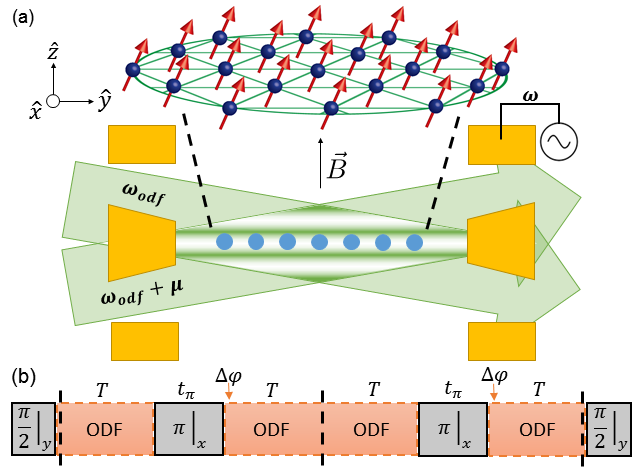
\includegraphics[width=\columnwidth]{expt}
    \caption{(a) Representation of ion spins arranged in a 2D triangular lattice, along with a cross-sectional illustration of the Penning trap, characterized by an axial magnetic field $B = 4.45$ T and an axial trap frequency $\omega_z = 2\pi \times 1.57$ MHz. The blue dots represent ions. Cylindrical electrodes (yellow) generate a harmonic confining potential along the $\hat{z}$-axis. Radial confinement is provided by the Lorentz force from $\vec{E} \times \vec{B}$-induced rotation in the axial magnetic field. The beams generating the spin-dependent optical dipole force (green arrows) cross the ion plane at $\pm 10^{\circ}$, forming a 1D traveling-wave potential (green lines) with a 0.9 $\mu$m wavelength. An AC voltage source is connected to the trap endcap and used to drive an axial oscillation with calibrated amplitude $Z_c$. (b) Quantum lock-in CPMG sequence used to detect spin precession produced by COM motion resonant with the ODF. Doppler cooling and $\ket{\uparrow}_N$ spin state preparation occur before the sequence, and spin state detection after. Grey blocks with solid borders represent microwave $\pi/2$ rotations about $\hat{y}$ and $\pi$ rotations about $\hat{x}$. Orange blocks with dashed borders represent ODF pulses. The ODF phase is advanced by $\Delta\varphi$ in a modulation scheme discussed in \citep{SuppMat}, where $\Delta\varphi = \pi$ for $\omega = \mu$. Dashed lines indicate the $m$ segments of the sequence, here $m = 2$. We make use of an $m = 8$ sequence for Figs. (2)-(4).} 
    \label{Expt}
\end{figure}

The ODF couples the spin and motional degrees of freedom through the interaction \citep{Bohnet2015}
\begin{equation}
\hat{H}_{ODF} = F_0\cos\left(\mu t \right)\sum_{i} \hat{z}_{i} \hat{\sigma}^{z}_{i},
\label{Hodf}
\end{equation}
where $F_0= U \, \delta k \, \rm{\it{DWF}}$ is the magnitude of the ODF, $\mu$ is the frequency difference between the ODF beams, and $\hat{z}_{i}$ and $\hat{\sigma}^{z}_{i}$ are the position operator and Pauli spin matrix for ion $i$. Here $U\:(\delta k)$ is the zero-to-peak potential (wave vector) of the 1D traveling-wave. The term $\rm{\it{DWF}} = \exp(-\delta k^2 \left< \hat{z}^{2}_{i} \right> / 2)$ is the Debye-Waller factor, a reduction in interaction strength due to the departure from the Lamb-Dicke confinement regime \citep{Wineland1998a}. We estimate $\rm{\it{DWF}} \approx 0.86 $ for the 0.5 mK Doppler laser cooling limit. The potential $U$, and therefore $F_0$, is determined from AC Stark shift measurements on the ions \citep{Britton2012}. Typical maximum values for this work are $U/\hbar \simeq 2 \pi \times (10.4$~kHz) resulting in $F_0 \simeq 40$ yN.

With a weak RF drive on a trap electrode (see Fig. \ref{Expt}(a)) at a frequency $\omega$ far from $\omega_{z}$, we impose a weak, classically driven COM motion of constant amplitude and phase, $\hat{z}_i \rightarrow \hat{z}_i +Z_c\cos(\omega t+\delta)$. With $\delta k Z_c \ll 1$ and assuming $\mu\sim\omega$, we use Eq. (\ref{Hodf}) to describe the shift in the spin transition frequency due to the coherent amplitude $Z_c$,
\begin{equation}
\hat{H}_{ODF} = F_{0} \, Z_c\cos((\omega - \mu)t + \delta) \sum_{i} \frac{\hat{\sigma}^{z}_{i}}{2} .
\end{equation}
For $\mu = \omega$ there is a static shift $\Delta(Z_c)$ in the frequency of the spin transition, $\Delta(Z_c) = (F_{0}/\hbar) \, Z_c \cos(\delta)$.

We measure $\Delta(Z_c)$ from the resulting spin precession in an experiment like that shown in Fig. \ref{Expt}(b). Ideally, spin precession can be measured using a Ramsey-type experiment where the ions are prepared in the $\ket{\uparrow}_N$ state, followed by a microwave $\pi/2$ pulse about $\hat{y}$ that rotates the spins to the $\hat{x}$ axis. The spins are then allowed to precess for an interaction time $\tau$ so that the resulting spin precession on resonance $(\mu = \omega)$ is $\theta = \theta_{max} \cos(\delta)$ where $\theta_{max} \equiv (F_{0}/\hbar)\, Z_c \, \tau$. After a final $\pi/2$ pulse about $\hat{y}$, the final state readout measures the population of the spins in $\ket{\uparrow}$, $P_{\uparrow} = \frac{1}{2}[1-e^{-\Gamma \tau}\cos(\theta)]$. Here $\Gamma$ is the decay rate from spontaneous emission from the off-resonant ODF laser beams \citep{Uys2010}. To detect small amplitudes with the available $F_0$ in our set-up, we extend the spin-precession time to $\tau \ge 20$ ms ($T \ge 1.25$ ms, in Fig. \ref{Expt}(b)). To avoid decoherence due to magnetic field fluctuations and coherently accumulate spin precession, we use a quantum lock-in \citep{Kotler2011} sequence where during the interaction time $\tau$ the spin precession is interrupted by a train of $\pi$-pulses that are synchronized with phase jumps enforced on the ODF beams \citep{SuppMat}. In particular, we use a Carr-Purcell-Meiboom-Gill (CPMG) sequence with $m = 8$ \mbox{ODF-$\pi$-ODF segments} (see Fig. \ref{Expt}(b)).

We allow the phase $\delta$ to randomly vary from one realization of the experiment to the next, effectively measuring a random quadrature of the motion each measurement trial. Such a scheme is relevant for sensing a force with an unknown or unstable phase. Different experimental trials therefore result in a different precession $\theta$, as indicated in Fig. \ref{Meas_stren}. We measure the collective dephasing (or decoherence) using $\left< P_{\uparrow} \right> = \frac{1}{2}[1-e^{-\Gamma \tau} \left<\cos(\theta)\right>]$, where the brackets $ \left< \cdot \right> $ denote an average over many measurements. Averaging over the random phase $\delta$ yields~\citep{Kotler2013}
\begin{equation}
\left< P_{\uparrow} \right> = \frac{1}{2} \left[ 1-e^{-\Gamma \tau}J_0(\theta_{max}) \right].
\label{Bessel}
\end{equation}
Here $J_0$ is the zeroth order Bessel function of the first kind.

To create the steady-state COM axial oscillation $Z_c \cos(\omega t+\delta)$, we applied a continuous AC voltage to an endcap of the Penning trap at a frequency $\omega/(2\pi)$ near 400 kHz. This frequency was chosen because it was far from any motional mode frequencies of the ion crystal, and there were no observed sources of noise. Thus, the background, i.e. the signal without the driven COM axial motion, was fully characterized by decoherence due to spontaneous emission and is given by $\left\langle P_{\uparrow}\right\rangle _{bck}= \frac{1}{2}\left[1-e^{-\Gamma\tau}\right]$. We calibrated the displacement of the ions due to a static voltage applied to the endcap by measuring the resulting movement of the ion crystal in the side-view imaging system. From this calibration, we determined that a 1 V offset results in a 0.97(5) $\mu$m displacement of the ions. We estimate that the corrections for using this DC calibration to estimate $Z_c$ for an $\omega/(2\pi) \approx 400$ kHz drive is less than 10$\,\%$.


Figure \ref{lineshape} shows the emergence of the measured spin precession signal out of the background as the amplitude $Z_c$ is increased from 500 pm to 5 nm. The measured lineshape agrees well with the prediction, detailed in \citep{SuppMat}, involving no free parameters.

\begin{figure}
    \centering
    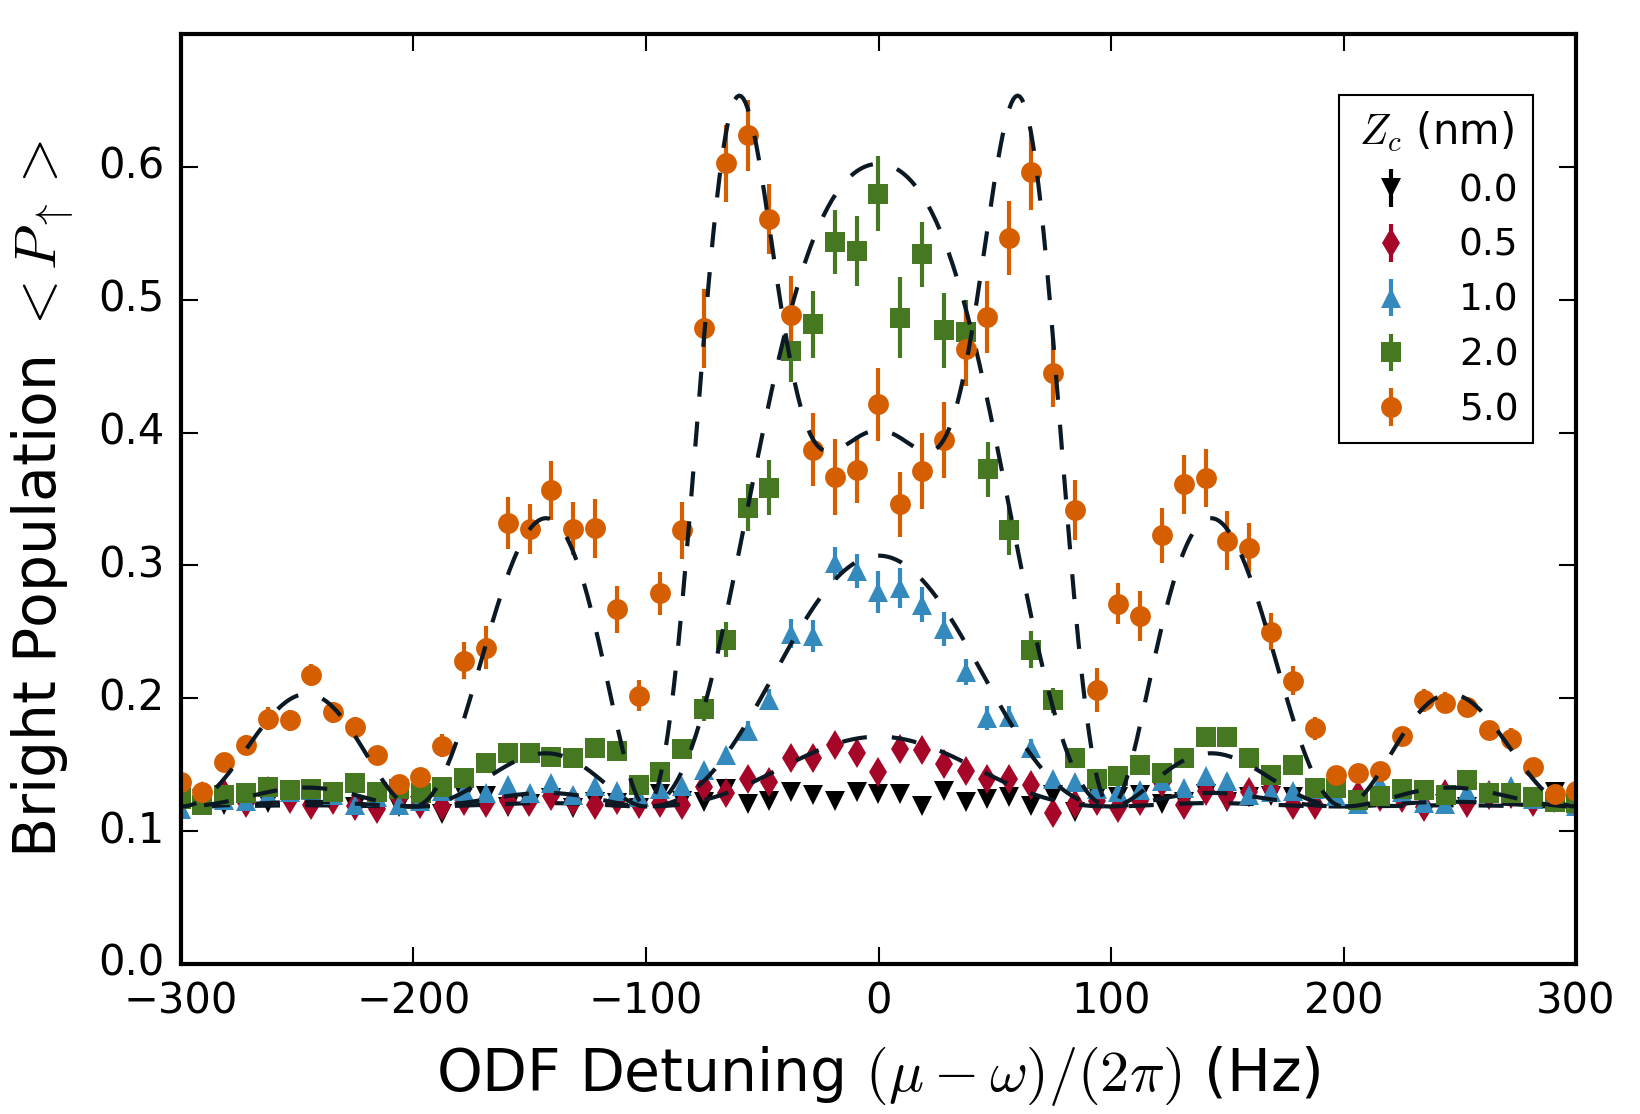
\includegraphics[width=\columnwidth]{lineshape}
  \caption{Lineshape of the spin precession signal for amplitudes $Z_c$ of 500 pm (red diamonds), 1 nm (blue triangles), 2 nm (green squares), and 5 nm (orange circles) for $\tau$ = 20 ms. Black triangles are the background, with the drive turned off. Dashed lines are theoretical predictions with no free parameters. Error bars represent standard error. Here $N = 90$ ions and $F_{0} = 7.9$ yN.}\label{lineshape}
\end{figure}

Figure \ref{Meas_stren} shows the background and the measured resonant ($\mu=\omega$) response to a fixed $Z_c$ = 485 pm oscillation for a range of ODF strengths $F_{0}/F_{0M}$, where $F_{0M}$ is the maximum $F_0$ possible with our current set-up ($\sim 40$ yN). Agreement with Eq. (\ref{Bessel}) involving no free parameters is excellent. For both Figs. \ref{lineshape} and \ref{Meas_stren} the background is within $6\,\%$ of that determined by independent measurements of the spontaneous emission decay rates of each ODF beam \citep{Britton2012}. The amplitude $Z_c=\theta_{max}/(\tau F_{0}/\hbar)$ can be determined from the difference $\left< P_\uparrow \right>- \left< P_\uparrow \right>_{bck}$. We note that $\left< P_\uparrow \right>- \left< P_\uparrow \right>_{bck}$ depends on $\theta_{max}^2$. Therefore, the sensing protocol described here directly measures $Z_c^2$. The inset of Fig. \ref{Meas_stren} shows a determination of $Z_c^2$ as the power in the ODF beams is increased. The uncertainties were determined from the measured noise of the $\left< P_\uparrow \right>- \left< P_\uparrow \right>_{bck}$ measurements using standard error propagation \citep{SuppMat}. These uncertainties go through a minimum, indicating an optimum $F_{0}/F_{0M}$ value for the determination of $Z_c^2$.
\begin{figure}
    \centering
    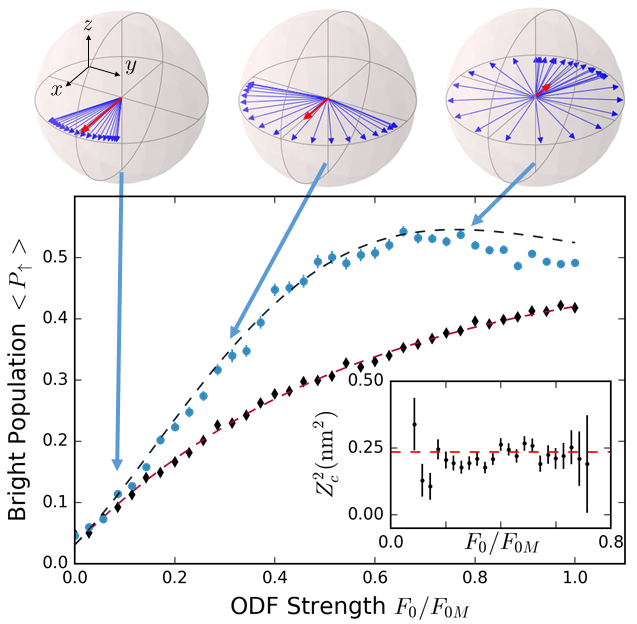
\includegraphics[width=\columnwidth]{odf_strength_bloch}
  \caption{\textbf{Top:} Bloch sphere representation \citep{QuTip} of spin dephasing for $Z_{c} = 485\: \rm{pm}$. Each blue vector represents an experimental trial with a different phase $\delta$ (see text). From left to right, the spread in the blue vectors corresponds to $\theta_{max} = 0.470, 1.41, 3.62$ radians and $F_{0}/F_{0M} = 0.1,0.3,0.77$, where $F_{0M}$ is the maximum optical-dipole force. Our experiment measures the length of the Bloch vector averaged over many trials, denoted by the thick red vector. \textbf{Main plot:} As a function of ODF strength, the background (black diamonds) with no applied drive and signal (blue points) for a 485 pm amplitude and total ODF interaction time $\tau$ = 24 ms is shown. The red dashed line is a fit to the background. The black dashed line is the theoretical prediction with no free parameters, given the background fit. Here $N = 75$ ions and $F_{0M} = 41.3$ yN. \textbf{Inset:} Black points are experimentally determined values for $Z_{c}^2$. Red dashed line is the calibrated value of $Z_{c}^{2}$. Error bars represent standard error.}\label{Meas_stren}
\end{figure}
\begin{figure}
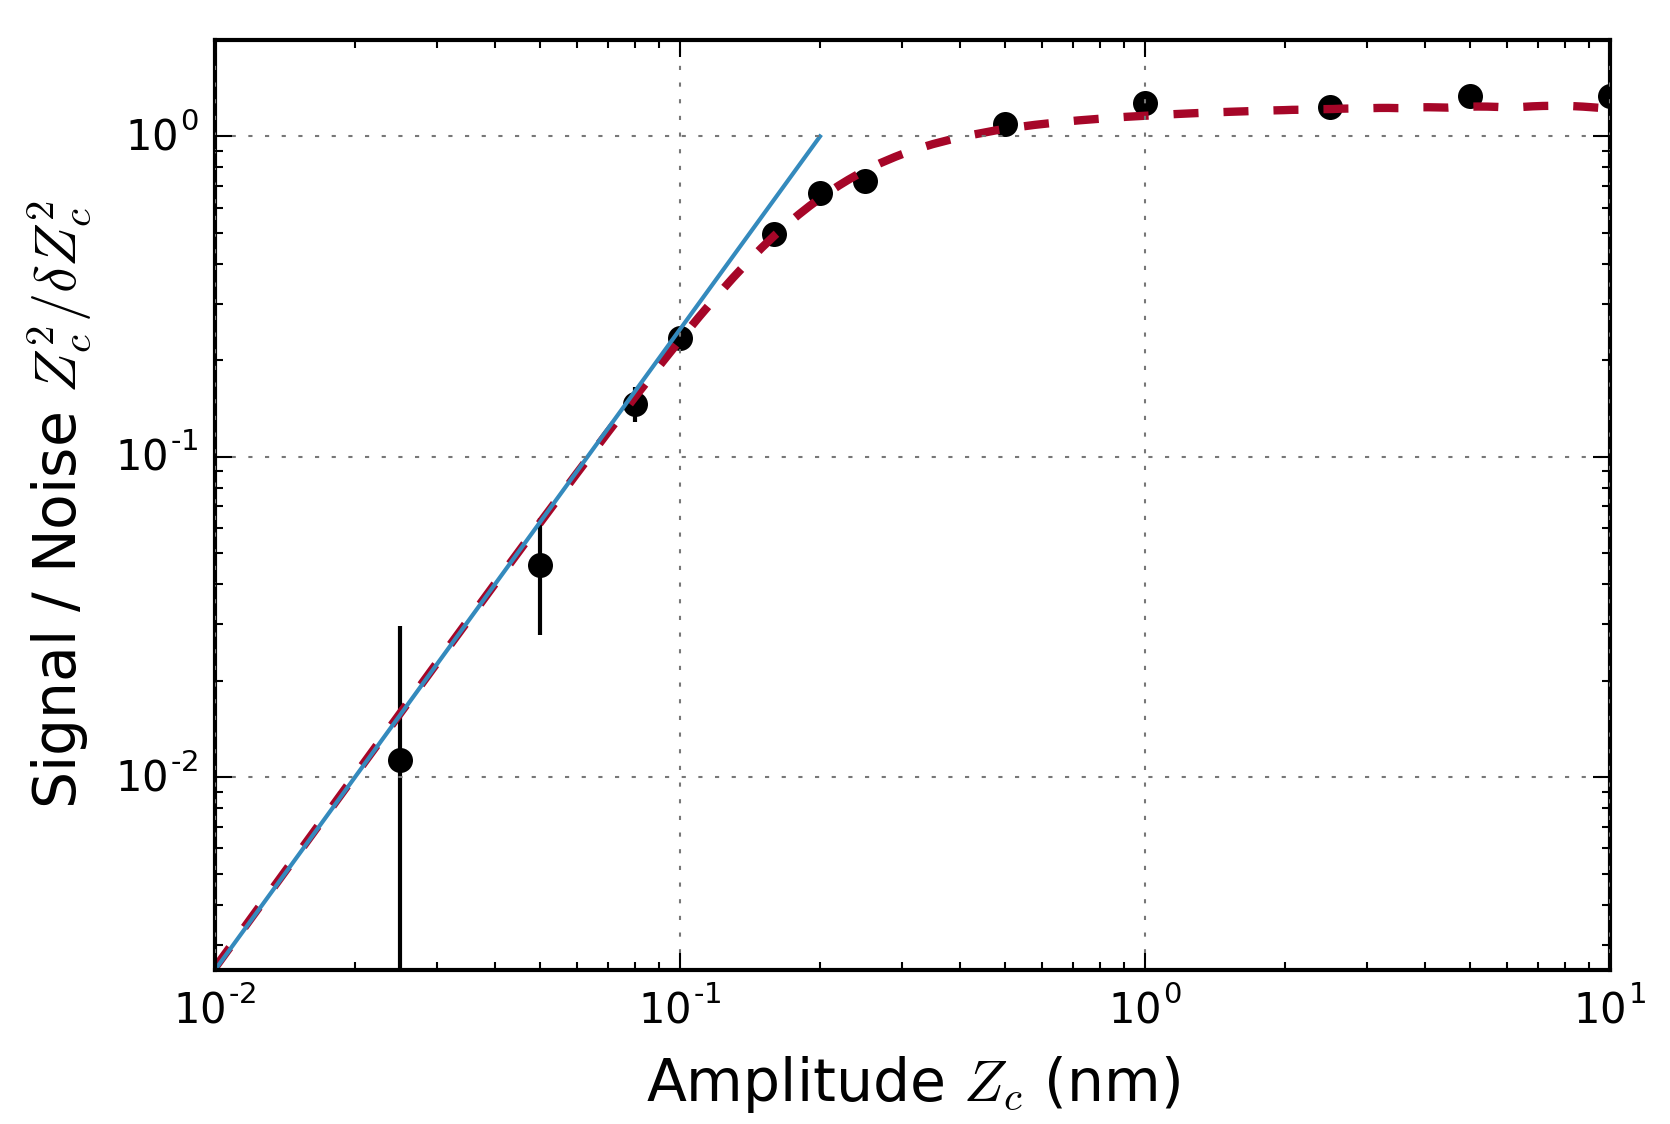
\includegraphics[width=\columnwidth]{sensing_limit}
\caption{Amplitude sensing limits for $N=85$. Black points are experimentally determined values of signal-to-noise for single measurements of $Z_{c}^{2}$ as a function of the experimentally imposed $Z_c$. Our measurement for $Z_c =$ 25 pm is consistent with zero. The red dashed line is the theoretical prediction for the signal-to-noise including projection noise and the random COM mode quadrature measured each trial. Blue solid line is the predicted limiting signal-to-noise for small amplitudes (Eq. (\ref{eq:limiting})), assuming only projection noise and parameters relevant for our set-up. Error bars represent standard error.} \label{Fig_sens}
\end{figure}

To explore the ultimate amplitude sensing limits of our protocol, we performed repeated pairs of $P_{\uparrow}$ measurements,
first with $Z_c = 0$ (i.e. no off-resonant drive on the trap endcap)
to get the background, and then with \mbox{$Z_{c}\neq0$}. For a given $Z_{c}$,
3,000 pairs of measurements were used to determine the average difference $\left\langle P_{\uparrow}\right\rangle -\left\langle P_{\uparrow}\right\rangle _{bck}$
and the standard deviation $\sigma\left( P_{\uparrow} - P_{\uparrow ,bck} \right)$
of the difference for a single pair of measurements. For each $Z_c$, $F_{0}/F_{0M}$ was set close to the value that maximizes the signal-to-noise ratio of
the $Z_{c}^{2}$ determination. This occurs for relatively small
$\theta_{max}$ such that \mbox{$\frac{1}{2}\left(1-J_{0}\left(\theta_{max}\right)\right)\approx\theta_{max}^{2}/8$}. Then, the signal-to-noise ratio of a determination of $Z_{c}^{2}$ from a single pair of $\ P_{\uparrow},\: P_{\uparrow, bck}$ measurements is approximately 
\begin{equation}
\frac{Z_{c}^{2}}{\delta Z_{c}^{2}}\approx\frac{\left\langle P_{\uparrow}\right\rangle -\left\langle P_{\uparrow}\right\rangle  _{bck}}{\sigma\left( P_{\uparrow} - P_{\uparrow , bck} \right)}\:.\label{eq:signal/noise}
\end{equation}
Figure \ref{Fig_sens} displays Eq. (\ref{eq:signal/noise}) from measurements acquired with $Z_{c}$
ranging from 10 nm to as small as 0.025 nm. Excellent agreement is
observed with a model (dashed red line) that assumes the only sources
of noise are projection noise in the spin state detection and fluctuations
in $P_{\uparrow}$ produced by random variation in the phase $\delta$ between the COM motion and the ODF from one measurement to the next.

For amplitudes $Z_{c}\gtrsim 500\:\mathrm{pm}$, noise due to different realizations of the phase $\delta$ dominates. This situation is depicted by the middle Bloch sphere of Fig. \ref{Meas_stren}. The fluctuations in $P_{\uparrow}$ due to different realizations of $\delta$ are comparable to the signal $\langle P_{\uparrow}\rangle - \langle P_{\uparrow} \rangle_{bck}$, limiting the signal-to-noise of a single measurement of $Z_{c}^{2}$
to ${\sim} 1$. As $Z_{c}$ decreases, this noise and the signal
decrease while projection noise stays approximately the same, resulting
in a decreasing $Z_{c}^{2}/\delta Z_{c}^{2}$. For small $Z_c$, we show the sensitivity is determined by $N$, $\delta k$, and the ratio of the spontaneous decay rate to the optical potential $\xi\equiv\Gamma/\left(U/\hbar\right)$ \citep{SuppMat}, according to
\begin{equation}
\left.\frac{Z_{c}^{2}}{\delta Z_{c}^{2}}\right|_{\mathrm{limiting}}\approx 0.097 \frac{\sqrt{N}(\rm{\it{DWF}})^2 (\delta k)^2}{\xi^2} Z_c^2\:.\label{eq:limiting}
\end{equation}
For $N=85$  and values of $\rm{\it{DWF}}$, $\delta k$, and $\xi=1.156\times10^{-3}$ relevant for our set-up, $Z_c^2/\delta Z_c^2 \approx \left[ Z_c/ 0.2 \, \rm{nm} \right]^2$, displayed as the blue line in Fig. \ref{Fig_sens}. On the log-log plot the slope of 2 is the result of a signal proportional to $Z_c^2$ along with a constant readout noise of the spins (here projection noise). We perform 16 measurements in 1 s, so the single measurement ${Z_{c}^{2}}/{\delta Z_{c}^{2}} \approx \left[ Z_c/ 0.2 \, \rm{nm} \right]^2$ corresponds to a long averaging time sensitivity of $\left(100\:\mathrm{pm}\right)^{2}/\sqrt{\mathrm{Hz}}$ (recall that our protocol measures $Z_{c}^2$).

Figure \ref{Fig_sens} documents a good understanding of the sensing limits
of our protocol, indicating how the measurement can be improved in the future.
Equation (\ref{eq:limiting}) scales as $1/\xi^{2}$, resulting in
significant improvements for set-ups with less spontaneous decay. By stabilizing the ODF beatnote phase with respect to the classical drive \citep{Hume2011, Biercuk2011}, or performing measurements conditioned on a pre-measurement designed to identify the relative phase between the ODF and classical drive, we could repeatedly measure the same quadrature of motion and realize a substantial improvement in sensitivity. 
For this phase-coherent protocol, we estimate \citep{SuppMat} a single measurement imprecision of 74 pm for $N=100$ and current parameters of our set-up, almost 30 times
smaller than the zero-point fluctuations, producing a long averaging time sensitivity of ${\sim}18\:\mathrm{pm/\sqrt{\mathrm{Hz}}}$. The use of spin-squeezed states, recently demonstrated in this system \citep{Bohnet2015}, can provide an additional enhancement by reducing the projection noise of the readout.

The 50 pm amplitude detected in Fig. \ref{Fig_sens} at a frequency $\omega$ far from resonance corresponds to an electric field detection of 0.46 mV/m or 73 yN/ion. These force and electric field sensitivities can be improved by the $Q$ of the COM mode by probing near resonance with $\omega_z$. Quality factors $Q\sim 10^6$ should be possible with trapped-ion COM modes. The detection of a 20 pm amplitude resulting from a 100 ms coherent drive on the 1.57 MHz COM mode is sensitive to a force/ion of $5\times10^{-5}\:\mathrm{yN}$ corresponding to an electric field of $0.35\:\mathrm{nV/m}$. Probing on resonance with a sensitivity below the zero-point fluctuations requires a protocol that evades back action due to coupling to thermal and quantum fluctuations \citep{Hempel2013}. Electric field sensing below ${\sim} \,0.1$ nV/m provides an opportunity to search for hidden photon dark matter \citep{Arias2012,Chaudhuri2015}, although shielding effects must be carefully considered. Ion traps typically operate with frequencies $\omega_z$ in the 50 kHz to 5 MHz range, providing a sensitivity to hidden photon masses in the $2 \times 10^{-10}$ eV to $2 \times 10^{-8}$ eV range.

In summary, we have presented a technique for amplitude sensing below the zero-point fluctuations of a trapped ion mechanical oscillator. By coupling
the spin and motional degrees of freedom of the ions, a single quadrature of the motional state of the ions may be sensitively read out. We implement a 
protocol where the phase of the measured quadrature randomly varies, detecting a 500 pm amplitude in a single measurement
and demonstrating a long measurement time sensitivity of $\left(100\:\mathrm{pm}\right)^{2}/\sqrt{\mathrm{Hz}}$. Modifications of our set-up should enable repeated measurements of a single quadrature, resulting in a single measurement
imprecision of 74 pm for $N = 100$ ions, providing opportunities for
trapped ion mechanical oscillators to explore the quantum limits of amplitude and force sensing, and enable new tools in the search for physics beyond the standard model.

\begin{acknowledgments}
We thank V. Sudhir, R. Ozeri, S. Kotler, and J. Teufel for stimulating discussions. K.G. is supported by NSF grant PHY 1521080. This manuscript is a contribution of NIST and not subject to U.S. copyright.
\end{acknowledgments}

\bibliographystyle{apsrev4-1}
\bibliography{amplitude_sensing}

\end{document}